\documentclass{article}

% if you need to pass options to natbib, use, e.g.:
%     \PassOptionsToPackage{numbers, compress}{natbib}
% before loading neurips_2021

% ready for submission
\usepackage[preprint]{neurips_2021}

% to compile a preprint version, e.g., for submission to arXiv, add add the
% [preprint] option:
%     \usepackage[preprint]{neurips_2021}

% to compile a camera-ready version, add the [final] option, e.g.:
%     \usepackage[final]{neurips_2021}

% to avoid loading the natbib package, add option nonatbib:
%    \usepackage[nonatbib]{neurips_2021}

\usepackage[utf8]{inputenc} % allow utf-8 input
\usepackage[T1]{fontenc}    % use 8-bit T1 fonts
\usepackage[colorlinks=true]{hyperref}       % hyperlinks
\usepackage{url}            % simple URL typesetting
\usepackage{booktabs}       % professional-quality tables
\usepackage{amsfonts}       % blackboard math symbols
\usepackage{nicefrac}       % compact symbols for 1/2, etc.
\usepackage{microtype}      % microtypography
\usepackage{xcolor}         % colors
\usepackage{graphicx}
\usepackage{subcaption}

\title{Predicting Student Performance\\ from Admissions and Historical Performance Data}

% The \author macro works with any number of authors. There are two commands
% used to separate the names and addresses of multiple authors: \And and \AND.
%
% Using \And between authors leaves it to LaTeX to determine where to break the
% lines. Using \AND forces a line break at that point. So, if LaTeX puts 3 of 4
% authors names on the first line, and the last on the second line, try using
% \AND instead of \And before the third author name.

\author{%
  Alexander Panfilov\\
  Matrikelnummer 5990087\\
  \texttt{alexander.panfilov@student.uni-tuebingen.de} \\
  \And
  Evgenii Kortukov\\
  Matrikelnummer 5994382\\
  \texttt{evgenii.kortukov@student.uni-tuebingen.de} \\
}

\begin{document}

\maketitle

\begin{abstract}
   We are planning to use a private dataset of anonymised data of ITMO University
   students. The dataset contains admission data (features such as entrance exam results,
   participation in math olympiads and demographic information) and performance from 
   previous semesters, such as average grade of all classes taken. We want to assess how well
   can student performance be predicted from this data. We are planning to use logistic and
   linear regression and also try dimensionality reduction techniques.
\end{abstract}

\section{Introduction}

\section{Data}
\begin{figure}[htb]
  \centering 
  \begin{subfigure}{0.49\textwidth}
    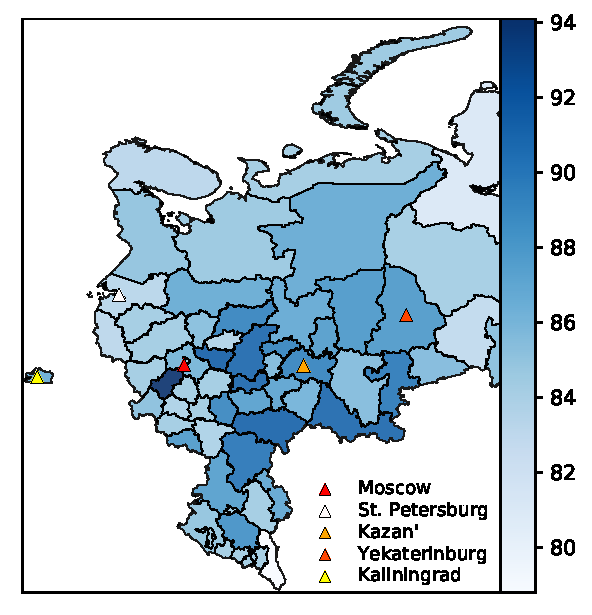
\includegraphics[width=\linewidth]{../gfx/map_informatics.pdf}
    \caption{Mean informatics state exam results}
    \label{fig:detection2d}
  \end{subfigure} 
  \begin{subfigure}{0.49\textwidth}
    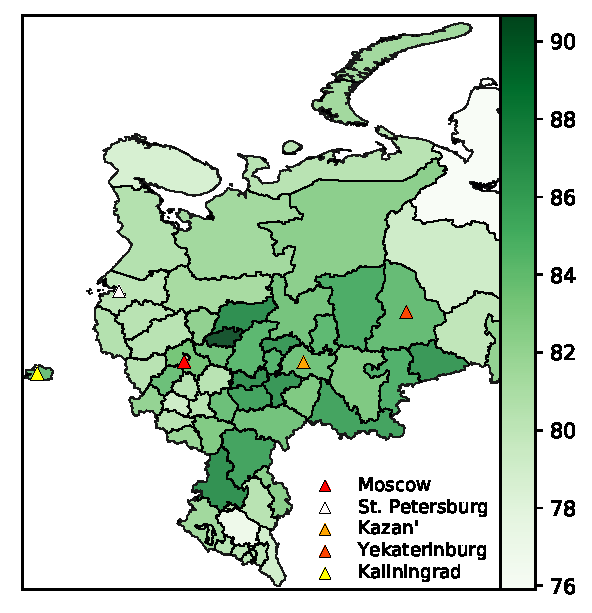
\includegraphics[width=\linewidth]{../gfx/map_math.pdf}
    \caption{Mean math state exam results}
    \label{fig:input}
  \end{subfigure}
  \begin{subfigure}{0.98\textwidth}
    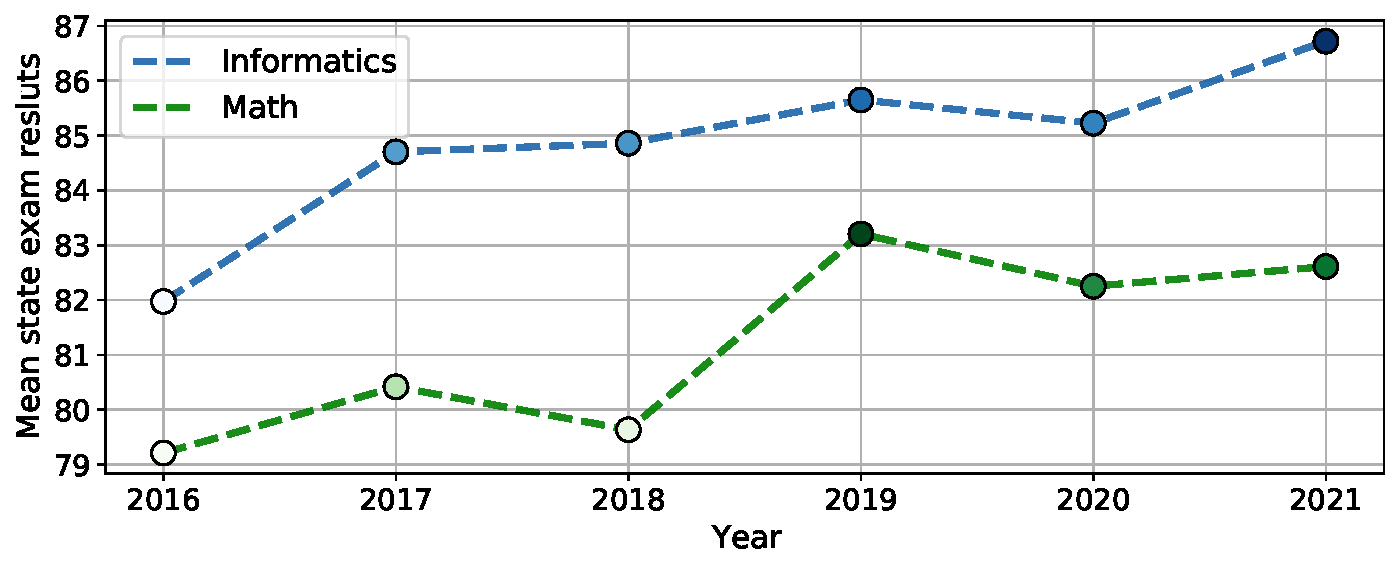
\includegraphics[width=\linewidth]{../gfx/ege_trend.pdf}
    \caption{Mean admitted state exam results over years}
    \label{fig:detection3D}
  \end{subfigure}\hfil

  \caption{\textbf{text}: }
\end{figure}

\section{Preprocessing}

\section{Hypothesis testing}

\section{Dimensionality reduction}

\begin{figure}[htb]
  \centering % <-- added

  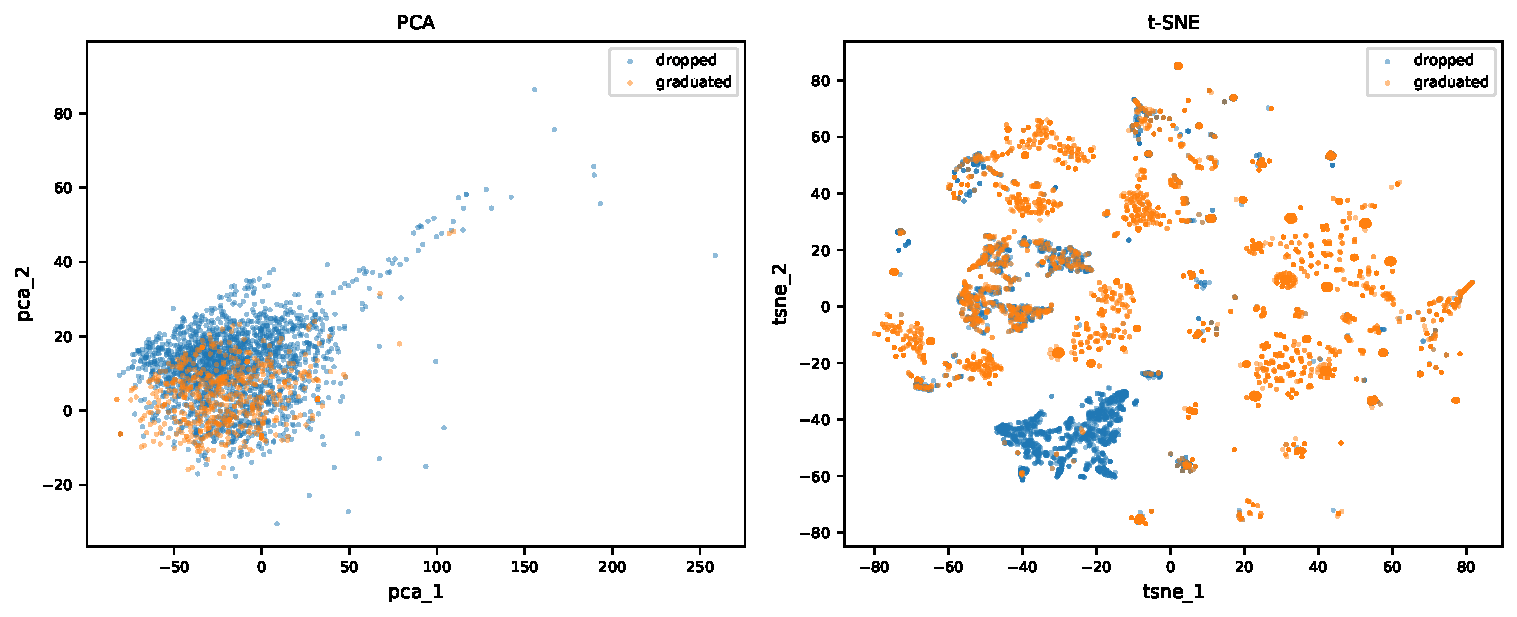
\includegraphics[width=1\linewidth]{../gfx/pca_tsne.pdf}
  \caption{pca}
  \label{fig:applot}
\end{figure}

\section{Regression}


\section{Ethics}


\section{Conclusion}


\end{document}
